\documentclass{standalone}

\usepackage{tikz}
\usetikzlibrary{shapes,arrows, decorations.markings}

\begin{document}
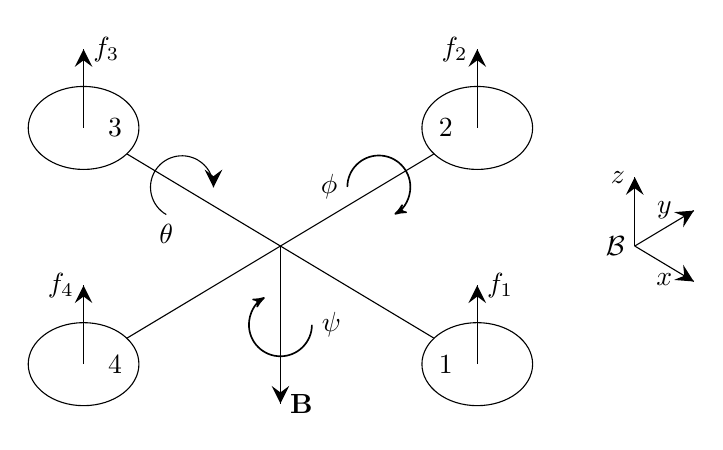
\begin{tikzpicture}
	\tikzstyle{prop} = [draw, ellipse, align=center, minimum width=4em, minimum height=3em]
	\tikzstyle{big_arrow} = [decoration={markings,mark=at position 1 with {\arrow[scale=2,>=stealth]{>}}},postaction={decorate}]
	% Prop nodes
	\node[prop, align=right] (1) at (0,0) {};
	\node[prop, align=left] (2) at (5,0) {};
	\node[prop, align=left] (3) at (5,3) {};
	\node[prop, align=right] (4) at (0,3) {};
	% Label props
	\node[draw=white, rectangle] at (4.6,0) {1};
	\node[draw=white, rectangle] at (4.6,3) {2};
	\node[draw=white, rectangle] at (0.4,3) {3};
	\node[draw=white, rectangle] at (0.4,0) {4};
	
	% Draw 
	% Connect props
	\draw [-] (1) -- node [midway, above] {} (3);
	\draw [-] (2) -- node [midway, above] {} (4);
		
	%Body Weight arrow 
	\draw [big_arrow] (2.5,1.5) -- node [at end, right] {\textbf{B}} (2.5,-0.5);
	% Prop thrust arrows
	\draw [big_arrow] (5,0) -- node [at end, right] {$f_1$}(5,1);
	\draw [big_arrow] (5,3) -- node [at end, left] {$f_2$} (5,4);
	\draw [big_arrow] (0,3) -- node [at end, right] {$f_3$}(0,4);
	\draw [big_arrow] (0,0) -- node [at end, left] {$f_4$} (0,1);
	
	% Draw arcs	
	\draw[big_arrow] (1.05,1.9) arc[radius=0.4, start angle=240, end angle=0] node[at start, below]{$\theta$};
	\draw[->,>=stealth',semithick] (3.35,2.25) arc[radius=0.4, start angle=180, end angle=-60] node[at start, left]{$\phi$};
	\draw[->,>=stealth',semithick] (2.9,0.5) arc[radius=0.4, start angle=0, end angle=-240] node[at start, right]{$\psi$};
	
	% Draw axes
	\draw [big_arrow] (7,1.5) -- node [midway, below] {$x$} (7.75,1.05);	
	\draw [big_arrow] (7,1.5) -- node [midway, above] {$y$} (7.75,1.95);
	\draw [big_arrow] (7,1.5) -- node [at end, left] {$z$} node [at start, left] {$\mathcal{B}$} (7,2.375);
	
\end{tikzpicture}

\end{document}